\section{Individual Path Finding}
\begin{frame}{Individual Path Finding}
    What is Individual Path finding?
    \begin{itemize}
        \item Creating \(n\) paths for each agents
        \item Creating \textbf{different kind of paths}
        \item Paths created do not consider collision with other paths
    \end{itemize}
    \begin{itemize}
        \item For each agent \(a\), we have \(\gamma_a\) = \(\{\pi_0,\dots,\pi_n\}\)
        \begin{itemize}
            \item \(\gamma\) is a set of paths
        \end{itemize}
        \item \(\tau\) representing the output of IPF 
        \begin{itemize}
            \item \(\tau = \{\gamma_a, \gamma_{a'}, ...\}\) is a set of set of paths
        \end{itemize}
    \end{itemize}
\end{frame}


\begin{frame}{IPF output example}
    \begin{figure}[H]
        \centering
        \caption{Example of a \(\tau = \{\gamma_r, \gamma_b, \gamma_g\}\)}\label{fig:ipf_example}
        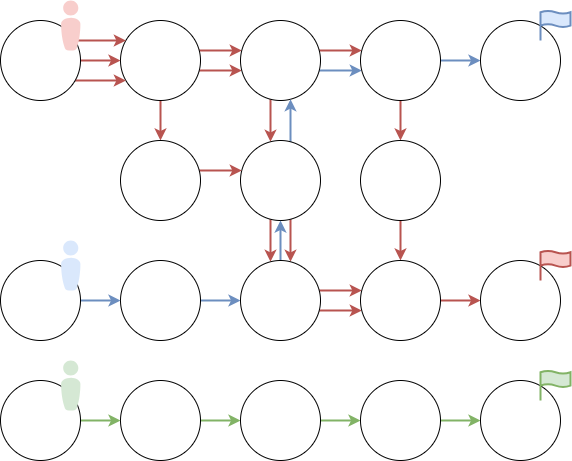
\includegraphics[width=7cm]{img/ipf_example.drawio.png}
    \end{figure}
\end{frame}



\subsection{IPF Computation}

\begin{frame}{Base IPF Computation}
    Principle of Base IPF computation
    \begin{figure}[H]
        \centering
        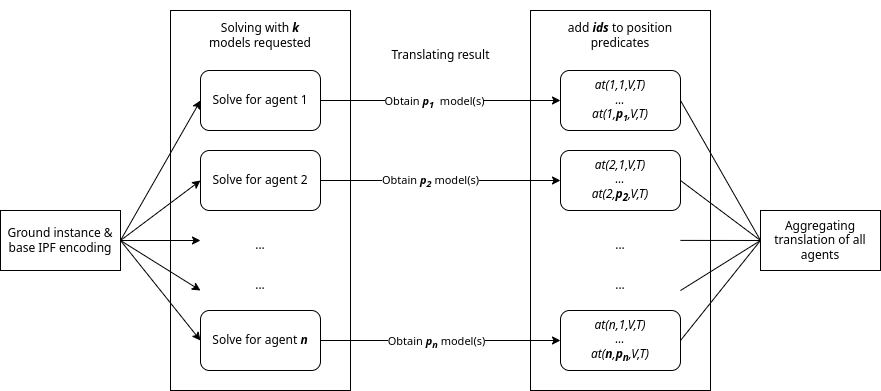
\includegraphics[width=11cm]{img/flowchart_ipf_computation.drawio.png}
    \end{figure}
\end{frame}
